
\subsection{Bewertungskriterien}
Die Beleuchtung soll durch einzelne LED-Pixel stattfinden. Ein Pixel bedeutet ein Chip auf dem sowohl die LED und der nötige Treiber sitzt. Für die Evaluierung werden folgende Kriterien gewählt:
\begin{itemize}
\item RGB-Farbraum \\
Die LED muss den gesamten RGB-Farbraum darstellen können. \\
Gewichtung: 5, KO-Kriterium
\item Ansteuerung \\
Da der Raspberry Pi an einigen seiner Pins Pulsweitenmodulation (PWM) bietet, sollten die LED-Pixel ohne extra Hardware ansteuerbar sein. Eine extra Stromversorgung ist aber bei größerer Anzahl an LEDs unabdingbar. \\
Gewichtung: 10
\item Framework \\
Hier wird bewertet ob der jeweilige Hersteller ein fertiges Framework zu seinen Produkten anbietet. \\
Gewichtung: 10
\item Kosten \\
Es werden nur die reinen Produktkosten, also ohne Versand und Zoll, bewertet. \\
Gewichtung: 5
\item Extras \\
An dieser Stelle können mögliche Extras eines Herstellers einfließen. \\
Gewichtung: 5
\end{itemize}

\subsection{Evaluierung}
\begin{itemize}
\item Adafruit, Neopixel \\
https://www.adafruit.com/neopixel \\
LED-Pixel in unzähligen Ausführungen. \\
Sitz der Firma in Tampa, Florida, USA \\
RGB: Chip ist der WS2801, http://www.adafruit.com/datasheets/WS2801.pdf -> Hat volle Abdeckung des RGB-Farbraums \\
Ansteuerung: Findet über PWM-Pin des Raspberry Pi statt. \\
Framework: Framework von Adafruit, welches eine sehr leichte Ansteuerung ermöglichen soll. \\
Kosten: 4 LEDs  7\$, 25 LEDs zusammen  39\$, durch Lieferung aus USA sehr hohe Versandkosten (50\$) \\
Extras: Händler bietet verschiedene Formen und fertige Ketten an. \\
\item LED-Emotion GMBH, LED Streifen \\
http://www.led-emotion.de/de/LED-Streifen-Set.html \\
LED-Streifen, keine Einzelpixel, nur mit Controller, keine API \\
RGB: Voller RGB-Farbraum \\
Ansteuerung: Nur mit Controller  \\
Framework: Keine öffentliche Api, möglicherweise mit Raspberry Pi ansteuerbar  \\
Kosten: 30 LEDs mit Netzteil 79€   \\
Extras: keine
\item DMX4ALL GmbH, MagiarLED Solutions \\
http://www.dmx4all.de/magiar.html \\
Spezialisiert auf DMX-Ansteuerung, keine öffentliche API \\
RGB: Volle Abdeckung RGB-Farbraum \\
Ansteuerung: Wird über DMX-Controller angesteuert, dieser setzt die Signale um. \\
Framework: DMX-Ansteurung über DMX-Controller \\
Kosten: Streifen mit 72 LEDs = 99€ \\
Extras: viele verschiedene Varianten
\item TinkerForge, RGB LED-Pixel \\
https://www.tinkerforge.com/de/shop/accessories/leds.html \\
Scheinen die gleichen wie von Adafruit zu sein, allerdings werden hauptsächlich Controller im Shop angeboten \\
RGB: Chip WS2801, volle Abdeckung RGB-Farbraum \\
Ansteuerung: Nach Anfrage an den Anbieter sollen die LEDs baugleich zu denen von Adafruit sein.  \\
Framework: keins, aber Ansteuerung über das Framework von Adafruit \\
Kosten: 50 LEDs = 59€ \\
Extras: Lieferung aus Deutschland
\end{itemize}
\begin{minipage}{\linewidth}
            \centering
            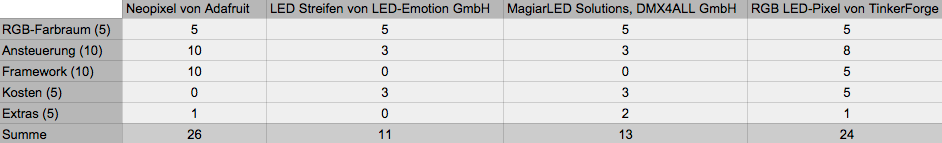
\includegraphics[width=\textwidth]{./data/evaluierung-led.png}
            \captionof{figure}{Ergebnisse der LED-Evaluierung}
        \end{minipage}
\paragraph{Fazit:}
In der Evaluierung schneiden die Produkte von Adafruit und TinkerForge am besten ab. Für eine erste Teststellung werden die einzelnen LED-Pixel von Adafruit aus den USA bestellt (Neopixel). An diesen soll vor allem die Ansteuerung getestet werden. Falls sie sich bewähren, wird für den endgültigen Aufbau auf die LED-Ketten von Tinkerforge zurück gegriffen. 

\subsection{Teststellung}
Für einen ersten Test wurde das in XXX ausgewählte Produkt als einzelne Pixel bestellt. Der Hersteller Adafruit bietet hier 4er-Packungen an. Diese können leicht in eigene Schaltungen eingelötet oder auf Experimentier-Boards gesteckt werden. Bei geringer Anzahl LEDs reicht die 5V-Stromversorgung des Raspberry Pi aus. 
\paragraph{Technische Daten Neopixel:} 
	\begin{itemize}
	\item Maße: 10.2mm x 12.7mm x 2.5mm
	\item Protokollgeschwindigkeit: 800 kHz
	\item Spannung: 5-9VDC  (bei 3,5V gedimmte Helligkeit) 
	\item Strom: 18,5mA / LED, 55mA / Pixel
	\end{itemize}
\paragraph{Framework:}
	\begin{itemize}
	\item RPI\_WS281X (https://github.com/jgarff/rpi\_ws281x)
	\item Sprache: Python
	\item Entwickelt für Raspberry Pi
	\item Vorraussetzung: Python 2.7
	\end{itemize}
\paragraph{Ablauf des Tests:}
\begin{itemize}

\item \textbf{Aufbau der Schaltung}\\
An die einzelnen LED-Pixel wurden Stecker angelötet, damit sie auf das Experimentierboard aufgesteckt werden können. Dann wird die Schaltung nach folgendem Schaltbild verbunden. Wichtig ist, dass beim Raspberry Pi nur Pins verwendet werden können, welche PWM\footnote{Pulsweitenmodulation: Signalübertragung durch Wechsel zwischen zwei Spannungen (High, Low), Breite des Impulses ist das Signal} bieten. \\
\begin{minipage}{\linewidth}
            \centering
            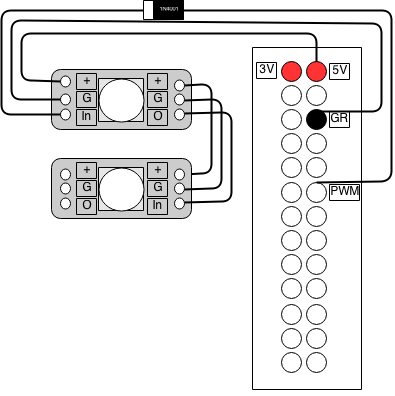
\includegraphics[width=8cm]{./data/TestSchaltungLED.png}
            \captionof{figure}{Schaltung für LED-Test}
        \end{minipage}
\item \textbf{Installation des Frameworks} 
\begin{lstlisting}[caption = Installation Framework ws281x, language=Python, frame=single, breaklines=true,columns=fullflexible, commentstyle=\color{gray}\upshape, captionpos=b, numbers = left]
wget https://github.com/tdicola/rpi_ws281x/raw/master/python/dist/rpi_ws281x-1.0.0-py2.7-linux-armv6l.egg 
sudo easy_install rpi_ws281x-1.0.0-py2.7-linux-armv6l.egg
\end{lstlisting}
\item \textbf{Testcode}

\begin{lstlisting}[caption = Testcode zur Ansteuerung der LEDs, language=python, frame=single, breaklines=true,columns=fullflexible, commentstyle=\color{gray}\upshape, captionpos=b, numbers = left]
from neopixel import * 
	
LED_COUNT   = 4       # Number of LED pixels. 
LED_PIN     = 18      # GPIO pin connected to the pixels (must support PWM!).
LED_FREQ_HZ = 800000  # LED signal frequency in hertz (usually 800khz)
LED_DMA     = 5       # DMA channel to use for generating signal (try 5)
LED_INVERT  = False   # True to invert the signal (when using NPN)

strip = Adafruit_NeoPixel(LED_COUNT, LED_PIN, LED_FREQ_HZ, LED_DMA, LED_INVERT)

strip.begin()
strip.setPixelColor(0, Color(255, 255, 255))
strip.setPixelColor(1, Color(255, 255, 255))
strip.setPixelColor(2, Color(255, 255, 255))
strip.setPixelColor(3, Color(255, 255, 255))
strip.show()
\end{lstlisting}
\end{itemize}
\paragraph{Fazit}
Die einzelnen Pixel sind sehr leicht anzusteuern, unterstützen auch das automatische Abschalten nach einer bestimmten Zeit und haben eine sehr hohe Leuchtkraft. Die Evaluierung hat zu einer guten Produktwahl geführt. \\ 
Nach einer weiteren Nachfrage an Tinkerforge wurde versichert, dass deren LED-Ketten Baugleich zu denen von Adafruit sind. Aufgrund der hohen Versandkosten werden für die endgültige Teststellung die Produkte von Tinkerforge gewählt.
